% Editable native-computation schematic, no measured spectra or invented scores.
\documentclass[tikz,border=0pt]{standalone}
\usepackage{fontspec}
\setsansfont{LiberationSans}[Path=../../shared/assets/,Extension=.ttf,UprightFont=*-Regular,BoldFont=*-Bold]
\usepackage{unicode-math}\setmathfont{Latin Modern Math}
\usetikzlibrary{arrows.meta,calc}
\definecolor{ink}{HTML}{0C0C0C}\definecolor{muted}{HTML}{63676B}\definecolor{accent}{HTML}{187E74}\definecolor{soft}{HTML}{EDF6F5}
\hyphenpenalty=10000\exhyphenpenalty=10000
\begin{document}
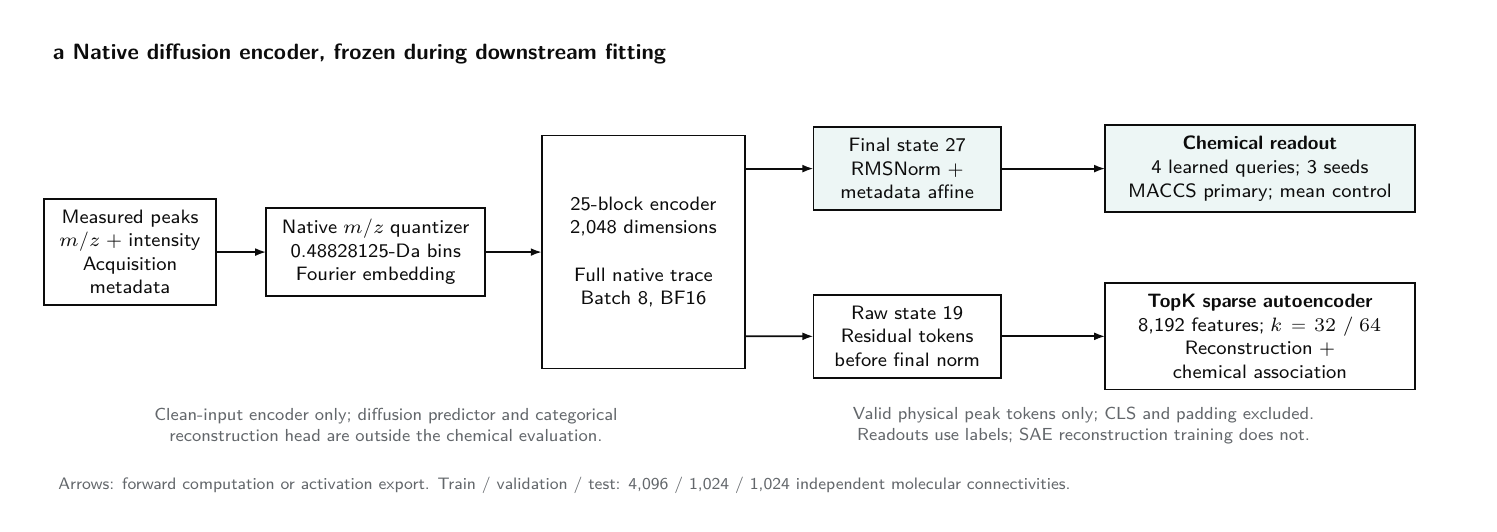
\begin{tikzpicture}[x=1cm,y=1cm,every node/.style={font=\sffamily\fontsize{7}{8.5}\selectfont,text=ink,align=center,inner sep=4pt,outer sep=0pt},box/.style={draw=ink,line width=.55pt,minimum height=1.05cm},flow/.style={-{Latex[length=1.4mm,width=1mm]},line width=.65pt,draw=ink},note/.style={font=\sffamily\fontsize{6.3}{7.6}\selectfont,text=muted}]
\path[use as bounding box] (0,0) rectangle (18.3,6.05);
\node[anchor=west,font=\sffamily\bfseries\fontsize{8}{10}\selectfont] at (.18,5.72) {a  Native diffusion encoder, frozen during downstream fitting};
\node[box,text width=1.90cm] (input) at (1.30,3.20) {Measured peaks\\$m/z$ + intensity\\Acquisition metadata};
\node[box,text width=2.50cm] (quant) at (4.42,3.20) {Native $m/z$ quantizer\\0.48828125-Da bins\\Fourier embedding};
\node[box,text width=2.30cm,minimum height=2.96cm] (enc) at (7.82,3.20) {25-block encoder\\2,048 dimensions\\\vspace{3mm}Full native trace\\Batch 8, BF16};
\node[box,text width=2.10cm,fill=soft] (final) at (11.17,4.26) {Final state 27\\RMSNorm +\\metadata affine};
\node[box,text width=3.65cm,fill=soft] (readout) at (15.65,4.26) {\textbf{Chemical readout}\\4 learned queries; 3 seeds\\MACCS primary; mean control};
\node[box,text width=2.10cm] (raw) at (11.17,2.13) {Raw state 19\\Residual tokens\\before final norm};
\node[box,text width=3.65cm] (sae) at (15.65,2.13) {\textbf{TopK sparse autoencoder}\\8,192 features; $k=32$ / $64$\\Reconstruction + chemical association};
\draw[flow] (input.east)--(quant.west);
\draw[flow] (quant.east)--(enc.west);
\draw[flow] ($(enc.east)+(0,1.06)$)--(final.west);
\draw[flow] ($(enc.east)+(0,-1.07)$)--(raw.west);
\draw[flow] (final.east)--(readout.west);
\draw[flow] (raw.east)--(sae.west);
\node[note,text width=7.2cm] at (4.55,1.00) {Clean-input encoder only; diffusion predictor and categorical\\reconstruction head are outside the chemical evaluation.};
\node[note,text width=8.45cm] at (13.41,1.00) {Valid physical peak tokens only; CLS and padding excluded.\\Readouts use labels; SAE reconstruction training does not.};
\node[anchor=west,note,font=\sffamily\fontsize{6}{7.2}\selectfont] at (.25,.24) {Arrows: forward computation or activation export. Train / validation / test: 4,096 / 1,024 / 1,024 independent molecular connectivities.};
\end{tikzpicture}
\end{document}
